\chapter{Results} % fixme

\section{Human3.6M}
\subsection{Evaluation protocol}
Human3.6M has 11 subjects out of which 7 are publically released while the rest are kept private. There are 2 widely used evaluation protocol. Protocol-1 is using all 4 camera views in subjects $S1$, $S5$, $S6$, $S7$ and $S8$ for training and the 
same 4 camera views in subjects $S9$ and $S11$ for validation/testing. Protocol-2 is the same as 1 expect that the predictions are post-processed via a rigid transformation
before comparing to the ground-truth.

% TODO Experiments

\subsection{2D-3D lifting}

The results presented are after training the model for ~1400 epochs on approximately 300,000 2D poses with a batch size of 2560 on a Titan X while flipping them with a probability of 0.5. The architecture is as described earlier with 1024 hidden units per linear layer and 512 latent dimensions. Both the \ac{vae} and the discriminator are trained using Adam optimizer with default hyperparameters, and with a learning rate of 2e-4. 

The different poses during the training are presented in fig. \ref{fig:sample_pred}. The poses in pink are the ground truth while the ones in blue are the predictions. The poses refer to ground truth 2D, reconstruction 2D, reconstruction novel view, reconstruction 3D and combined reconstruction and ground truth 3D after alignment. The same order is followed for the other visualization. 

\begin{figure}[!h]
    \centering
    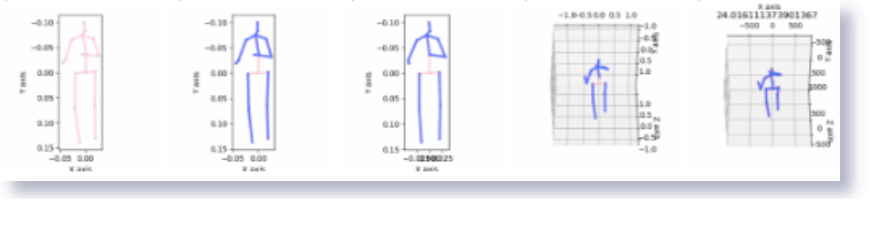
\includegraphics[scale=0.4]{figures/sample_pred.png}
    \caption{Visualization of the inputs and outputs of the model}
    \label{fig:sample_pred}
\end{figure}

One of the challenging parts is finding the optimal weights for each of the terms in the triplet loss. The $\beta$ value for the \ac{bvae} is cycled from 0 to 0.001 for every 40 epochs while keeping it constant at 0.001 for 10 epochs with a 10 epoch warmup at the beginning of the training. The weight of the critic with scaling the magnitudes is 1e-4. While the weight for the reconstruction loss is kept at 1. 

The discriminator is trained for 3 iterations for one iteration of the \ac{vae}. The training is noise and the networks need to training for several hundreds of epochs before they tend to converge. The experiment which the results are from, is trained over 1400 epochs but very slow improvements in the results are observed. At 1400 epochs the \ac{mpjpe} is ~68 mm. This is far less than the current state of the art \cite{amazon1} with ~40 mm. The results are believed to improve using \acp{wgan} as they offer better convergence. 

Despite the \ac{mpjpe} being ~68, the decoder generates many accurate 3D poses that are almost indistinguishable for the human eye. The high number of outlier and lower performace on hard poses worsens the overall performace of the model. The graph on the left depicted in fig \ref{fig:mpjpe_trends} shows the slow and gradual decrease in \ac{mpjpe}. And the graph on the right shows the histogram of the \ac{pjpe} of each sample over time. This shows the model is unable to certain poses while it improves gradually on the rest. 

\begin{figure}[!h]
    \centering
    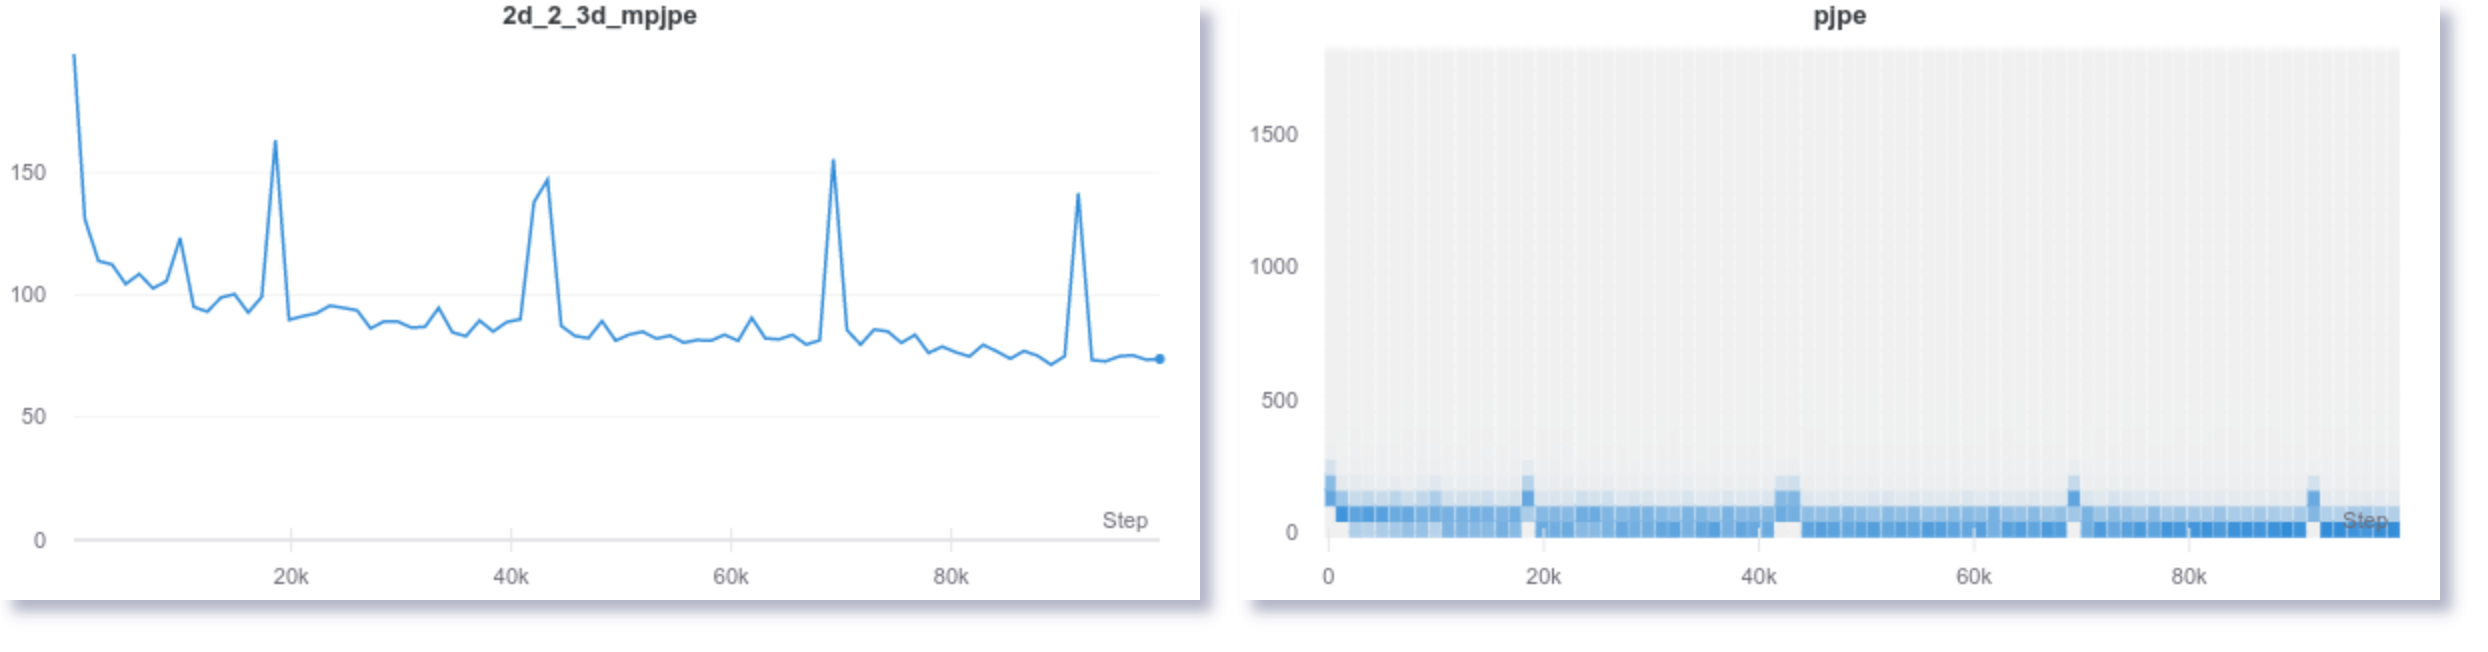
\includegraphics[scale=0.2]{figures/mpjpe_trend.png}
    \caption{MPJPE and PJPE trends during the training respectively}
    \label{fig:mpjpe_trends}
\end{figure}

Some of such outliers are presented in fig \ref{fig:bad_samples}, the predictions in (a) are the ones the model is unable to learn. While (b) is the evidence of the shortcoming of the current processing technique. Rectifing that would imporve the evaluation metric of the model quite significantly.

\begin{figure}[!h]
    \centering
    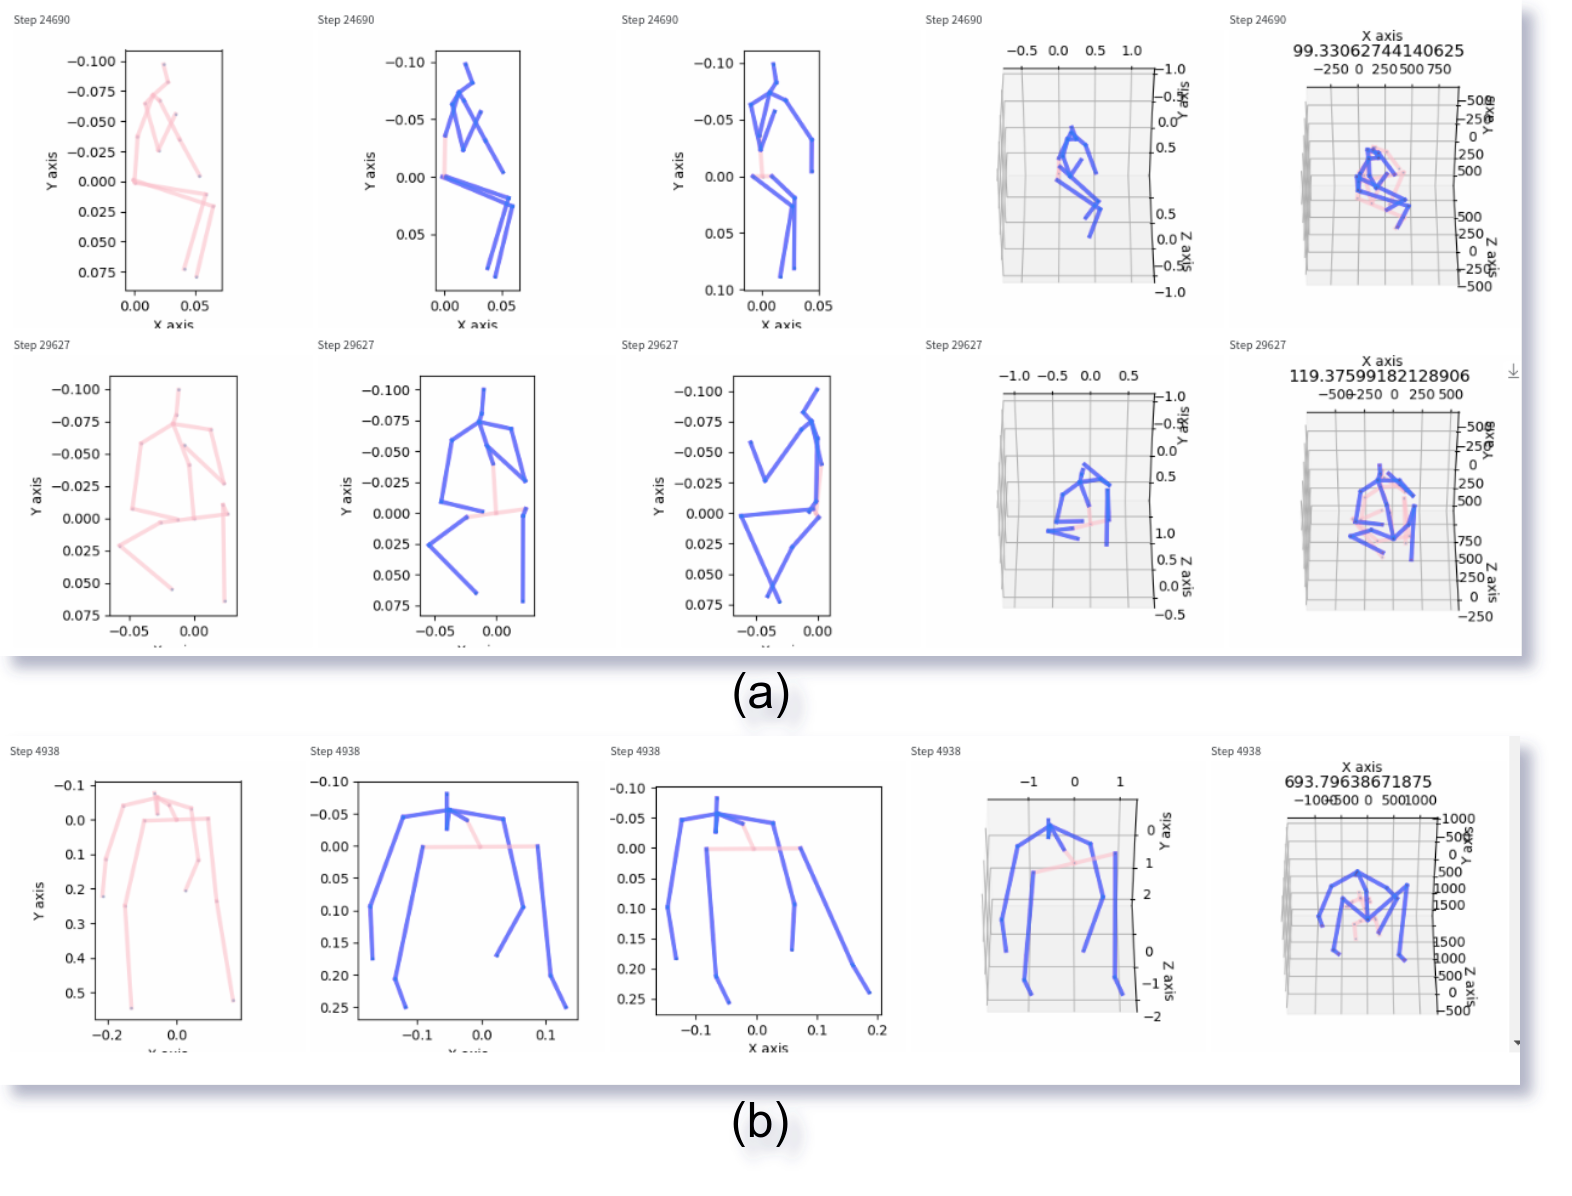
\includegraphics[scale=0.2]{figures/bad_samples.png}
    \caption{(a) Prediction on hard poses with hih ambiguity. (b) Poses that can be improved with changes to data processing.}
    \label{fig:bad_samples}
\end{figure}



The visualization of 2D pose embedding in latent space after dimensionality reduction using \ac{umap} is shown in 
fig. \ref{fig:latentspace}. Each action is given a unqiue color. Though we small clusters of blues, browns, pinks the overall space looks very mixed up. This is expected as many of the instance in different actions overlap. For example, the action standing up and sitting down have instances while both or standing or sitting etc.  

\begin{figure}[h]
    \centering
    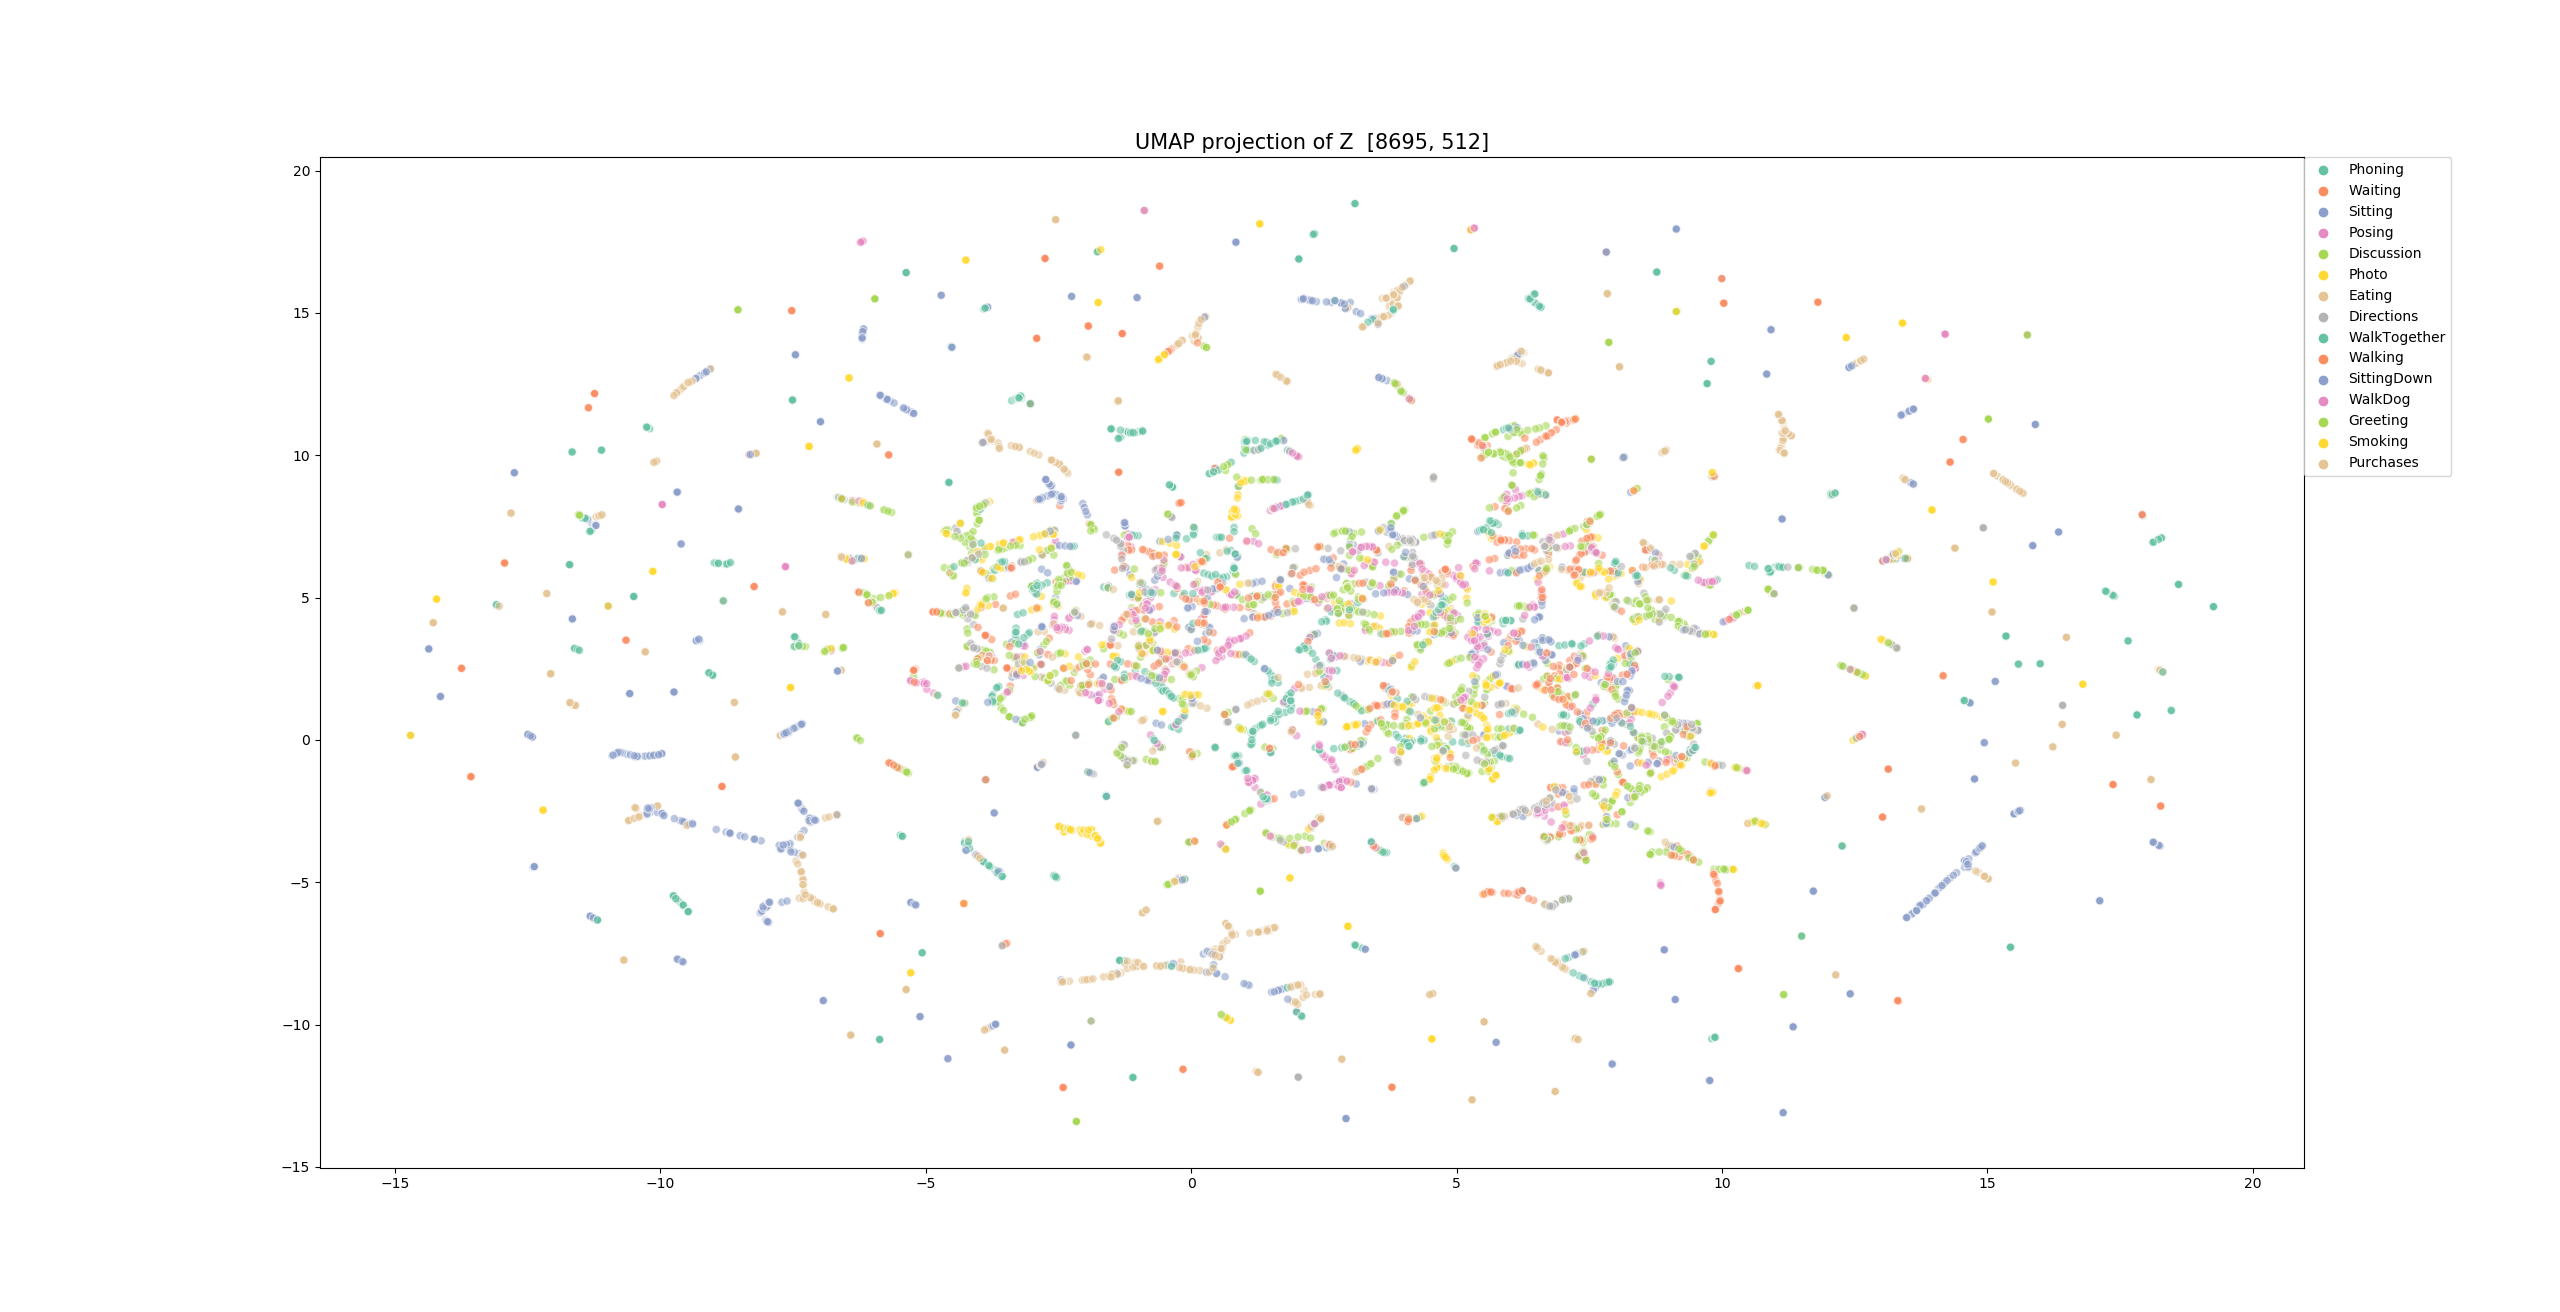
\includegraphics[width=\textwidth]{figures/umap.png}
    \caption{UMAP Visualization of samples in latent space. The actions do not always directly related to the pose due to overlaps from one action to another.}
    \label{fig:latentspace}
\end{figure}